%!TEX program = xelatex
\documentclass[a4paper,UTF8]{article}
\usepackage{ctex}
\usepackage[margin=1.25in]{geometry}
\usepackage{color}
\usepackage{graphicx}
\usepackage{amssymb}
\usepackage{amsmath}
\usepackage{amsthm}
\usepackage{enumerate}
\usepackage{bm}
\usepackage{hyperref}
\usepackage{epsfig}
\usepackage{color}
\usepackage{mdframed}
\usepackage{lipsum}
\usepackage{graphicx}
\usepackage{float}
\newmdtheoremenv{thm-box}{Theorem}
\newmdtheoremenv{prop-box}{Proposition}
\newmdtheoremenv{def-box}{定义}

\usepackage{listings}
\usepackage{xcolor}
\lstset{
	numbers=left,
	numberstyle= \tiny,
	keywordstyle= \color{ blue!70},
	commentstyle= \color{red!50!green!50!blue!50},
	frame=shadowbox, % 阴影效果
	rulesepcolor= \color{ red!20!green!20!blue!20} ,
	escapeinside=``, % 英文分号中可写入中文
	xleftmargin=2em,xrightmargin=2em, aboveskip=1em,
	framexleftmargin=2em
}

\usepackage{booktabs}

\setlength{\evensidemargin}{.25in}
\setlength{\textwidth}{6in}
\setlength{\topmargin}{-0.5in}
\setlength{\topmargin}{-0.5in}
% \setlength{\textheight}{9.5in}
%%%%%%%%%%%%%%%%%%此处用于设置页眉页脚%%%%%%%%%%%%%%%%%%
\usepackage{fancyhdr}
\usepackage{lastpage}
\usepackage{layout}
\footskip = 12pt
\pagestyle{fancy}                    % 设置页眉
\lhead{2020年秋季}
\chead{神经网络}
% \rhead{第\thepage/\pageref{LastPage}页}
\rhead{作业一}
\cfoot{\thepage}
\renewcommand{\headrulewidth}{1pt}  			%页眉线宽,设为0可以去页眉线
\setlength{\skip\footins}{0.5cm}    			%脚注与正文的距离
\renewcommand{\footrulewidth}{0pt}  			%页脚线宽,设为0可以去页脚线

\makeatletter 									%设置双线页眉
\def\headrule{{\if@fancyplain\let\headrulewidth\plainheadrulewidth\fi%
\hrule\@height 1.0pt \@width\headwidth\vskip1pt	%上面线为1pt粗
\hrule\@height 0.5pt\@width\headwidth  			%下面0.5pt粗
\vskip-2\headrulewidth\vskip-1pt}      			%两条线的距离1pt
 \vspace{6mm}}     								%双线与下面正文之间的垂直间距
\makeatother

%%%%%%%%%%%%%%%%%%%%%%%%%%%%%%%%%%%%%%%%%%%%%%
\numberwithin{equation}{section}
%\usepackage[thmmarks, amsmath, thref]{ntheorem}
\newtheorem{theorem}{Theorem}
\newtheorem*{definition}{Definition}
\newtheorem*{solution}{Solution}
\newtheorem*{prove}{Proof}
\newcommand{\indep}{\rotatebox[origin=c]{90}{$\models$}}

\usepackage{multirow}

%--

%--
\begin{document}
\title{神经网络\\
作业五}
\author{181220076, 周韧哲, zhourz@smail.nju.edu.cn}
\maketitle

\section*{Problem 1}
Batch normalization的输出服从什么样的分布(指出分布中的具体参数)。
\begin{solution}服从标准正态分布$\mathcal{N}(0,1)$,均值为$0$,方差为$1$。
\end{solution}

\section*{Problem 2}
Batch normalization为什么归一化后还有放缩($\gamma$)和平移($\beta$)?
\begin{solution}
	$\gamma$和$\beta$的引入是为了恢复数据本身的表达能力,对规范化后的数据进行线性变换,即$\hat{x}=\gamma x+\beta$,就是变换的反操作,特别地,当$\gamma=\sigma,\beta=\mu$时,可以实现等价变换,并且保留了原始输入特征的分布信息。
\end{solution}
\section*{Problem3}
目前有一批病人的身体数据(体重变化,血液指标等)和他们是否患有肺癌的真实标签,其中患肺癌的样本只占非常小的比例。数据直接送入一个神经网络中,求问应该使用什么样的初始化?数据中不同的特征数值差异过大,求问如何改进能够让网络更好地学习数据中地分布?
\begin{solution}
	可以使用高斯分布初始化。数据中不同的特征数值差异过大可以使用$\text{Batch Normalization}$把每一层网络的输入数据规范化为均值为$0$方差为$1$的正态分布,能够缓解特征数值差异过大对网络造成的不良影响从而使得网络能够更好地学习数据分布。
\end{solution}
\section*{Problem4}
对神经网络损失函数添加正则化后形式如下,这里V为损失函数,R为正则化函数,给定输入$x_i$,神经网络输出为$f(x_i)$,$y_i$为真实标记。$$\min_f\sum_{i=1}^{n}V(f(x_i),y_i)+\lambda R(f)$$
\begin{enumerate}[(1)]
	\item 请说明参数$\lambda$的意义。
	\item 参数$\lambda$的取值是越大越好还是越小越好,请结合playground(https://playground.tensorflow.org)上面的实例说明理由。(注:在playground上,红框选中的区域用于选择正则化函数的种类以及设置参数$\lambda$的大小。)
\end{enumerate}
\begin{solution}.
	\begin{enumerate}[(1)]
		\item $\lambda$是正则化系数,用来调整损失项和正则项之间的系数,控制着$R(f)$的重要程度。随着$\lambda$的增大,$R(f)$的限制越强,对模型复杂性的惩罚因子就越大。
		\item $\lambda$越小,其惩罚项值不大,容易出现过拟合现象;$\lambda$越大,过拟合现象的程度越来越低,但是当$\lambda$的值超过一个阈值时,就会出现欠拟合现象,因为其惩罚项太大,导致丢失太多的特征,甚至一些比较重要的特征。因此,$\lambda$不是越大越好或者越小越好,它是一个超参数,需要根据问题实例来调整。如下图\ref{Fig:1}\ref{Fig:2}\ref{Fig:3},正则化系数分别为$0.001,0.1,0.3$,$0.3$时完全欠拟合,网络没有学到任何东西。
			\begin{figure}[!htb]
			\centering
			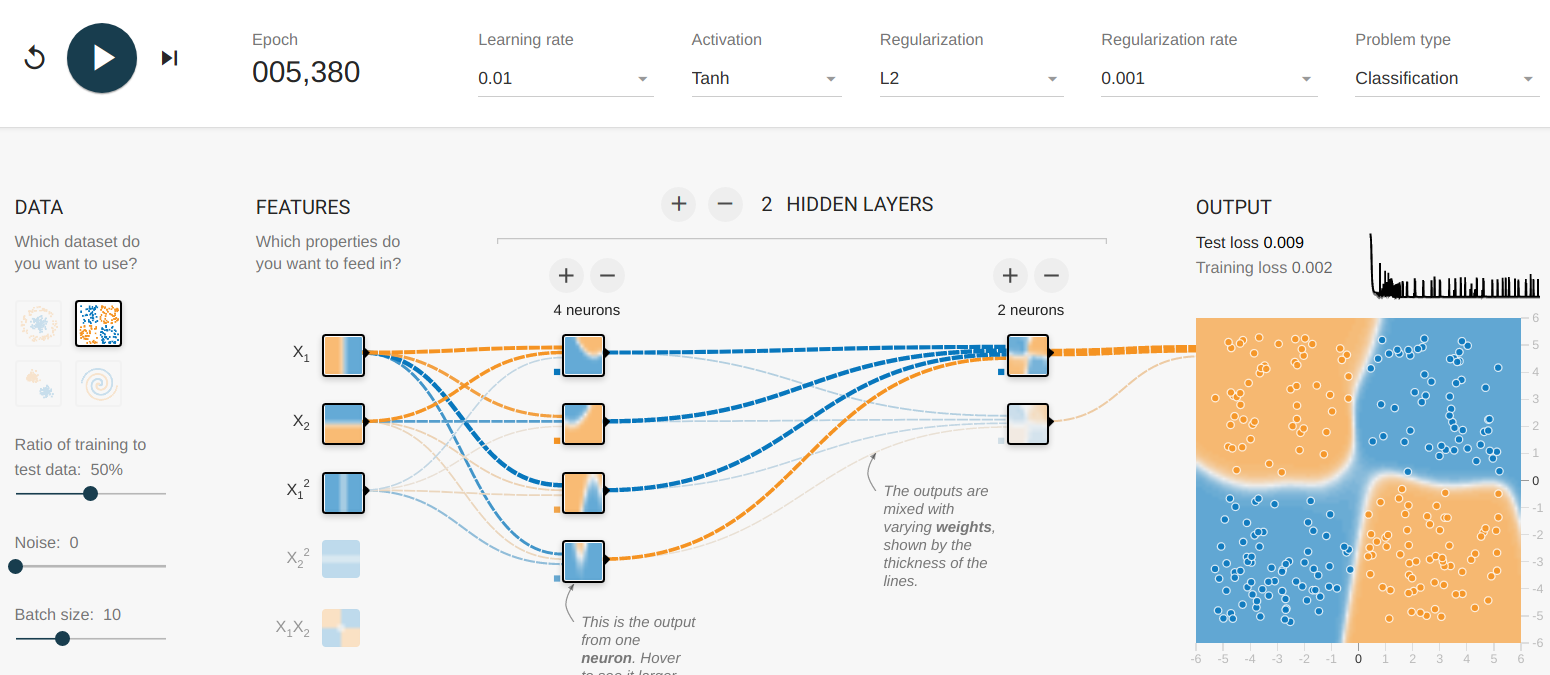
\includegraphics[width=1\textwidth]{pic/3.png}
			\label{Fig:1}
			\caption{0.001}
		\end{figure}
		\begin{figure}[!htb]
			\centering
			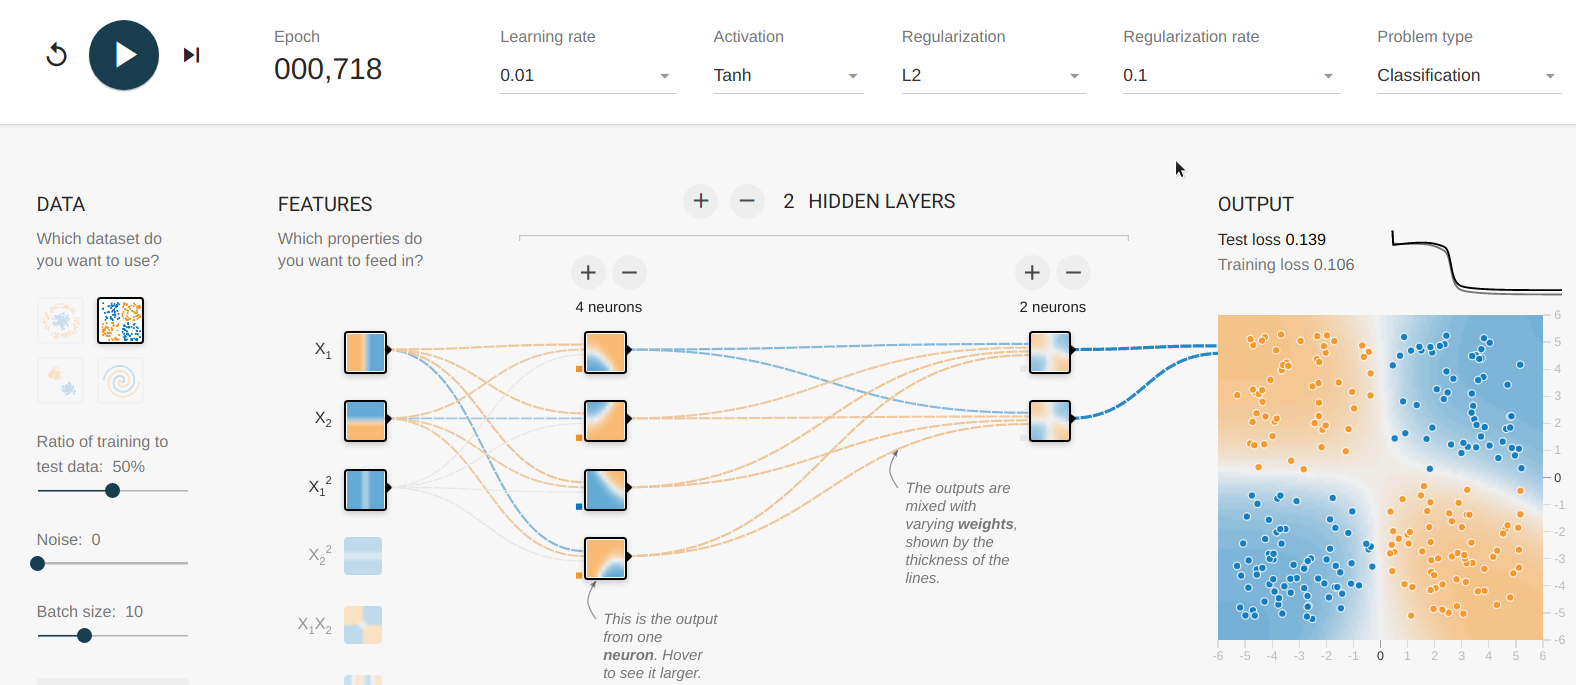
\includegraphics[width=1\textwidth]{pic/1.png}
			\label{Fig:2}
			\caption{0.1}
		\end{figure}
		\begin{figure}[!htb]
			\centering
			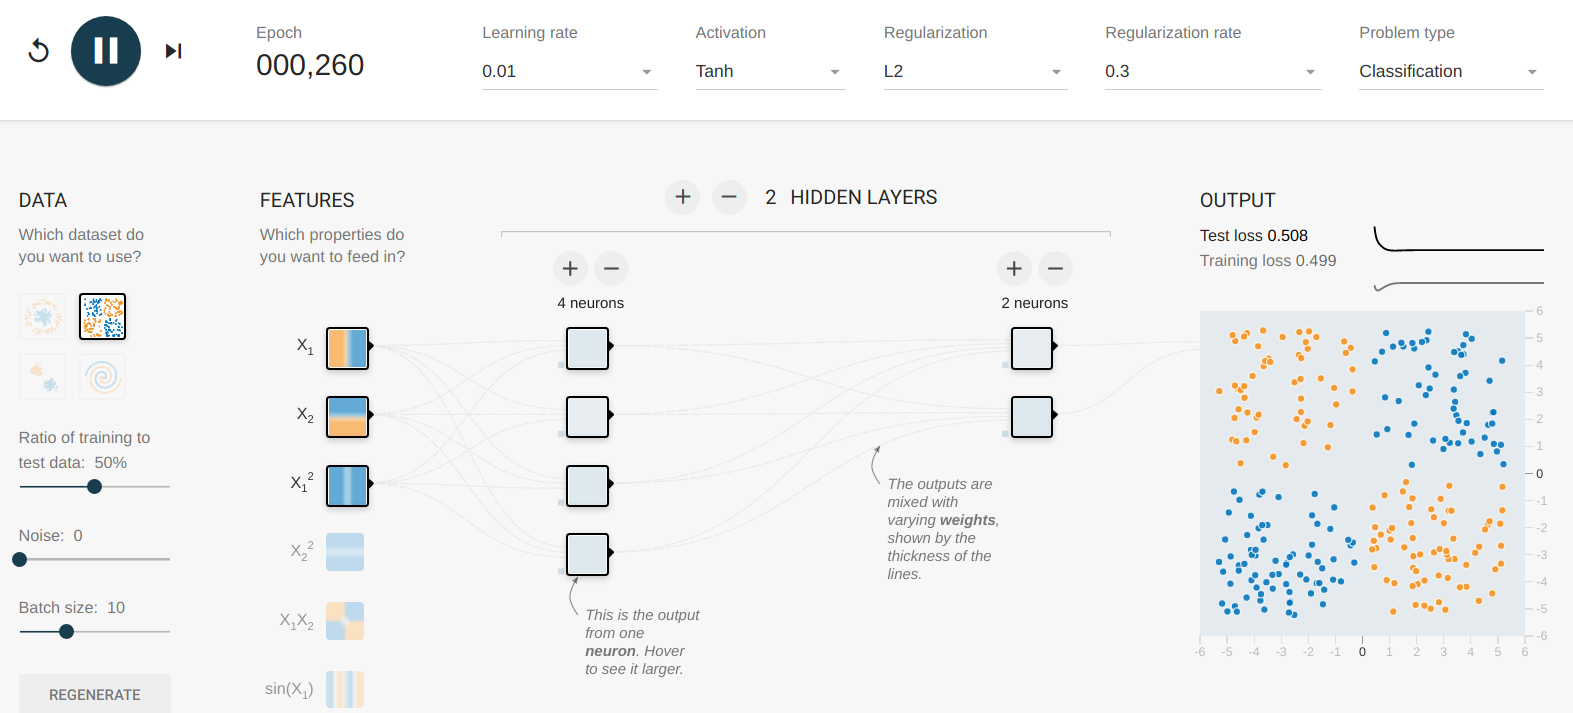
\includegraphics[width=1\textwidth]{pic/2.png}
			\label{Fig:3}
			\caption{0.3}
		\end{figure}
	\end{enumerate}
\end{solution}

\end{document}